\documentclass[12pt]{report}
\usepackage[utf8]{inputenc}
\usepackage[T1]{fontenc}
\usepackage[english]{babel}
\usepackage{graphicx}
\usepackage{amsmath}
\usepackage{amssymb}
\usepackage{hyperref}
\usepackage{epsf}
\usepackage{float}
\usepackage{geometry}
\geometry{hmargin=3.5cm, vmargin=2.5cm}
\usepackage[squaren]{SIunits}
\usepackage{listings}
\usepackage{color}
\definecolor{mygreen}{RGB}{70, 180, 90}
\definecolor{mylilas}{RGB}{255, 117, 45}
\definecolor{cadr}{rgb}{0.89, 0.0, 0.13}
\graphicspath{{DWGs/}}
\usepackage{graphicx}
\usepackage{wrapfig}
\usepackage{graphicx}
\usepackage{multicol}
\usepackage{enumitem}
\usepackage{xcolor}
\usepackage{framed}
\definecolor{listinggray}{gray}{0.9}
\definecolor{lbcolor}{rgb}{0.95,0.95,0.95}
\definecolor{shadecolor}{RGB}{179, 229, 184}

\begin{document}

\lstset{
		backgroundcolor=\color{lbcolor},
   		tabsize=4,    
    	language=C++,
        basicstyle=\sffamily,
        upquote=true,
        aboveskip={1.5\baselineskip},
        columns=fixed,
        showstringspaces=false,
        extendedchars=false,
        breaklines=true,
        numbers=left,
        showtabs=false,
        showspaces=false,
        showstringspaces=false,
        identifierstyle=\ttfamily,
        keywordstyle=\color[rgb]{0,0,1},
        commentstyle=\color[rgb]{0.026,0.5,0.095},
        stringstyle=\color{mylilas},
        numberstyle=\color{black},
		emph={for, break, if, while},
		emphstyle={\color{red}\textbf},
}



\begin{titlepage}
    \begin{center}

		\vspace*{5cm}    

        \Huge
        \textbf{Objectif Morse}
        
        \vspace*{0.5cm}

		\Large

		\textbf{
		\text{-}\text{-}\text{-} \,			%O
		$\cdot\cdot$\text{-} \,\,\,\,\,\,	%U
		$\cdot\cdot\cdot\cdot$ \,			%H
		$\cdot\cdot$ \,						%I
		$\cdot\cdot\cdot$ \,				%S
		\text{-} \,							%T
		\text{-}\text{-}\text{-} \,			%O	
		$\cdot\cdot$ \,						%I
		$\cdot$\text{-}$\cdot$ \,			%R
		$\cdot$}							%E
		
		\textbf{
		\text{-}$\cdot\cdot$ \,				%D
		$\cdot\cdot$\text{-} \,				%U
		\text{-}$\cdot$ \,\,\,\,\,\,		%N
		$\cdot$\text{-} \,					%A
		$\cdot$\text{-}$\cdot\cdot$ \, 		%L
		$\cdot$\text{-}$\cdot\cdot$ \, 		%L
		$\cdot$ \,							%E
		$\cdot$\text{-}$\cdot$}				%R
		
		\textbf{
		$\cdot$ \,							%E
		\text{-} \,\,\,\,\,\,				%T
		$\cdot$\text{-}$\cdot$	\,			%R
		$\cdot$ \,							%E
		\text{-} \,							%T
		\text{-}\text{-}\text{-} \,			%O
		$\cdot\cdot$\text{-} \,				%U
		$\cdot$\text{-}$\cdot$}				%R
		

        \vspace{2cm}
        
        \LARGE
        J. Aleksanderek
        
        K. Zdybal

        \vspace{8.5cm}
        
		\Large

 		January, 2017
	\end{center}
\end{titlepage}

\thispagestyle{empty}
\begin{center}
    
\vspace*{4cm}


\includegraphics[width = 70mm]{ex_libris.png}

\vspace*{2cm}

Copyright \textcopyright \, J. Aleksanderek, K. Zdybał, 2017

For more projects similar to this one

visit us on GitHub: @camillejr

To contact us personally drop us a line at:

\verb|kamilazdybal@gmail.com|

\end{center}
\newpage




\setlength{\parindent}{0cm}
\clearpage

\tableofcontents

\setlength{\parskip}{1em}
\renewcommand{\baselinestretch}{1.0}

\chapter{Introduction}\label{chap:intro}

\textbf{Welcome to the Objectif Morse project.} 

You will soon begin a journey through secret coded messages transmitted between powerful computers over tiny distances. 

The main purpose of this document is to keep the record of the ideas that we had, of the solutions that we came up with and of the observations that we have made. 

The second purpose is to serve as a tutorial for you, if you ever feel like embarking on the same adventure as we did. It is not very difficult! Following it, you will be able to (hopefully) accomplish the same mission! This journey will increase your knowledge in C++, Linux, Arduino, electronics and, undoubtedly, French language. Some basic understanding in all of these is requried as a prerequisite.

All the codes produced are not included in this document. You can download everything needed from the \href{https://github.com/camillejr/objectif_morse}{GitHub repository}.

Reach out to section [\ref{sec:equip}] to check if you have everything that you will need!

It's time to present the mission objectives...

\section{Voici l'Objectif Morse}

The idea for this project was born while reading \href{https://fr.wikipedia.org/wiki/Objectif_Lune}{Tintin} comic books. 

We have created the problem as follows:

You type a secret message on a stationary computer into the terminal. This message is translated into Morse alphabet and the signal of dots and dashes is sent to the parallel port as high and low states. The parallel port's pins are connected to a small circuit with an LED diode, which blinks accordingly to the message translation. No spies should be observing the diode. This message is received by a phototransistor, situated in the close proximity of the LED. The phototransistor pass on the signal to the Arduino device. Arduino connected to a portable computer prints the received message on the Serial Monitor. The message is translated by reading the Arduino output and printed again in the terminal of the portable computer. The message is received and the war is won.


\section{Project phases}

This project is divided into two phases: \textbf{broadcasting} and \textbf{receiving}. 

In general, these two phases don't require each other to get them working, however, the \textbf{receiving} phase needs a light trigger to obtain a signal. If you didn't build the  \textbf{broadcasting} phase, you can use the light e.g. from a flashlight. Nevertheless, it's not recommended from the debugging point of view, unless you are an expert in broadcasting Morse signals by hand.

The two phases are separated by a 1\textit{mm} air gap. What happens inside of the air gap shall forever remain a secret.


\section{Equipment used} \label{sec:equip}

Here is the list of all the equipment that we have used.

ELECTRONICS:

\begin{enumerate}

\item LED blue diode
\item phototransistor
\item resistors: 330, 10 000 Ohm
\item a few cables
\item breadboard
\item parallel port plug with soldered cables
\item piece of paper (I know, that doesn't really count as electronics)

\end{enumerate}

COMPUTATION:

\begin{enumerate}

\item Arduino Uno with a USB A-B cable
\item stationary computer with Linux ()
\item portable computer with Linux (Ubuntu)
\item of course you need some monitors and keyboards...

\end{enumerate}

OPTIONAL (increases the interactivity of this project):

\begin{enumerate}

\item flashlight

\end{enumerate}





\newpage

\chapter{Broadcasting}

\verb|OBJECTIF_MORSE, PHASE: BROADCASTING -| The first phase of the Objectif Morse project is to translate the secret message from the regular text to the Morse code. This part introduces the message input using alphanumeric characters in the terminal, where the corresponding program is running. The message is translated by the program and broadcasted on an LED diode connected to the parallel port output pin.

\section{Code description}

The Objectif Morse project is coded in C++ language. It utilises the most powerful part of C++: object-oriented programming.

The code for broadcasting the coded message consists of 5 files plus a makefile. 

The code is split into operating on the messages (\verb|morse.cpp| and \verb|morse.h|) and into sending output on the parallel port (\verb|sendToPort.cpp| and \verb|sendToPort.h|).

The most important constituents of each file are presented in the graph below.

\begin{figure}[H]
\centering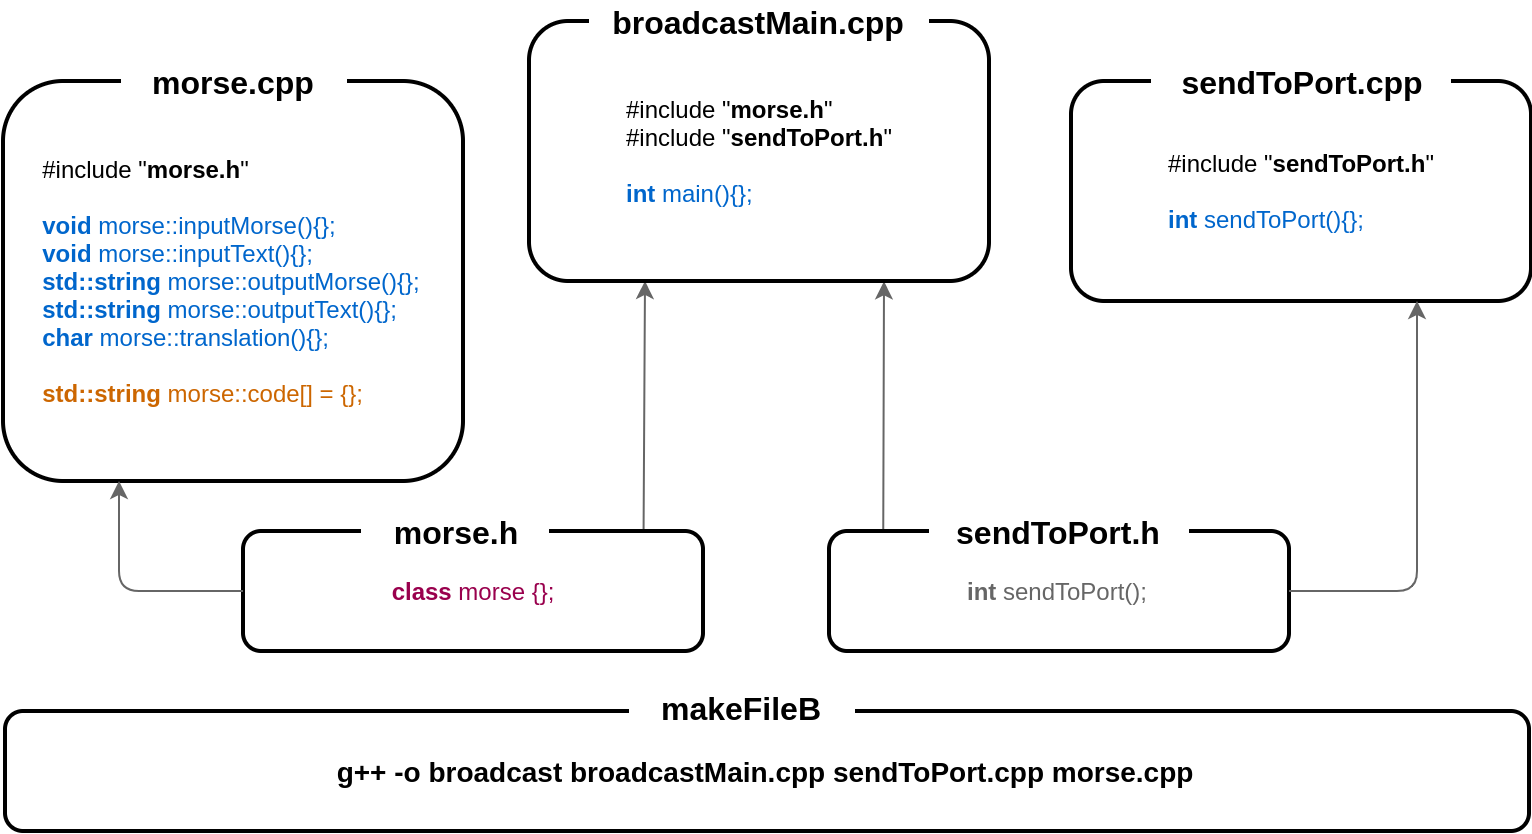
\includegraphics[scale=0.12]{bCodeStructure}
\caption{Code structure for \textbf{broadcasting} phase.}				
\label{fig:br_code}
\end{figure}




\subsection{Class morse}

We created a class called \verb|morse| that handles all the necessary variables and functions corresponding to translating from \verb|text > morse| and from \verb|morse > text|.

The definition of the class is presented in the listing \ref{App:morse_h}. We will now describe the class elements.

We start with the class functions:

\rule{\textwidth}{0.5pt}

\verb|morse::inputMorse()| - a public function that takes a string written in Morse alphabet as an input. Ideally, the input string should only consist of the following characters:

\begin{enumerate}
\item dot \verb|"."|

\item dash \verb|"-"|

\item space \verb|" "|

\item slash \verb|"/"|
\end{enumerate}

If the user inputs characters other then the listed above, they will be treated as unknowns in the message.

\rule{\textwidth}{0.5pt}


\verb|morse::inputText()| - a public function that takes a string written in alphanumeric as an input. The input string should only consist of:

\begin{enumerate}
\item letters \verb|A-Z| (\verb|a-z|)
\item numbers \verb|0-9|
\item space \verb|" "|
\item dot \verb|"."|
\item comma \verb|","|
\end{enumerate}

If the user inputs characters other then the listed above, they will be treated as unknowns in the message.

\rule{\textwidth}{0.5pt}

\verb|morse::outputMorse()| - 

\rule{\textwidth}{0.5pt}

\verb|morse::outputText()| - 

\rule{\textwidth}{0.5pt}

\verb|morse::translation()| - 

\rule{\textwidth}{0.5pt}



Following are the class variables:

\rule{\textwidth}{0.5pt}

\verb|morse::morseMessage| - is a private string that contains a message written in the Morse alphabet.

\rule{\textwidth}{0.5pt}

\verb|morse::textMessage| - is a private string that contains a message written in the alphanumeric characters.

\rule{\textwidth}{0.5pt}

\verb|morse::code| - is a private array of strings. A closer description of this array is given in section [\ref{sec:asciitomorse}]

\rule{\textwidth}{0.5pt}

\subsection{Functions}










\subsection{Sending output to the parallel port}



\subsection{Main}



\subsection{Makefile}

To compile the code on your computer you can use the following makefile:




\section{How does it work}

\newpage

\subsection{Parallel port}

In this section we describe how to connect to the parallel port and how to build a simple circuit with an LED diode. Notice that not every computer has got a parallel port! Usually, a modern portable computer will not be equiped with a parport, so try to get one oldschool stationary computer like we did! The parallel port is big and pink like this one:

\begin{figure}[H]
\centering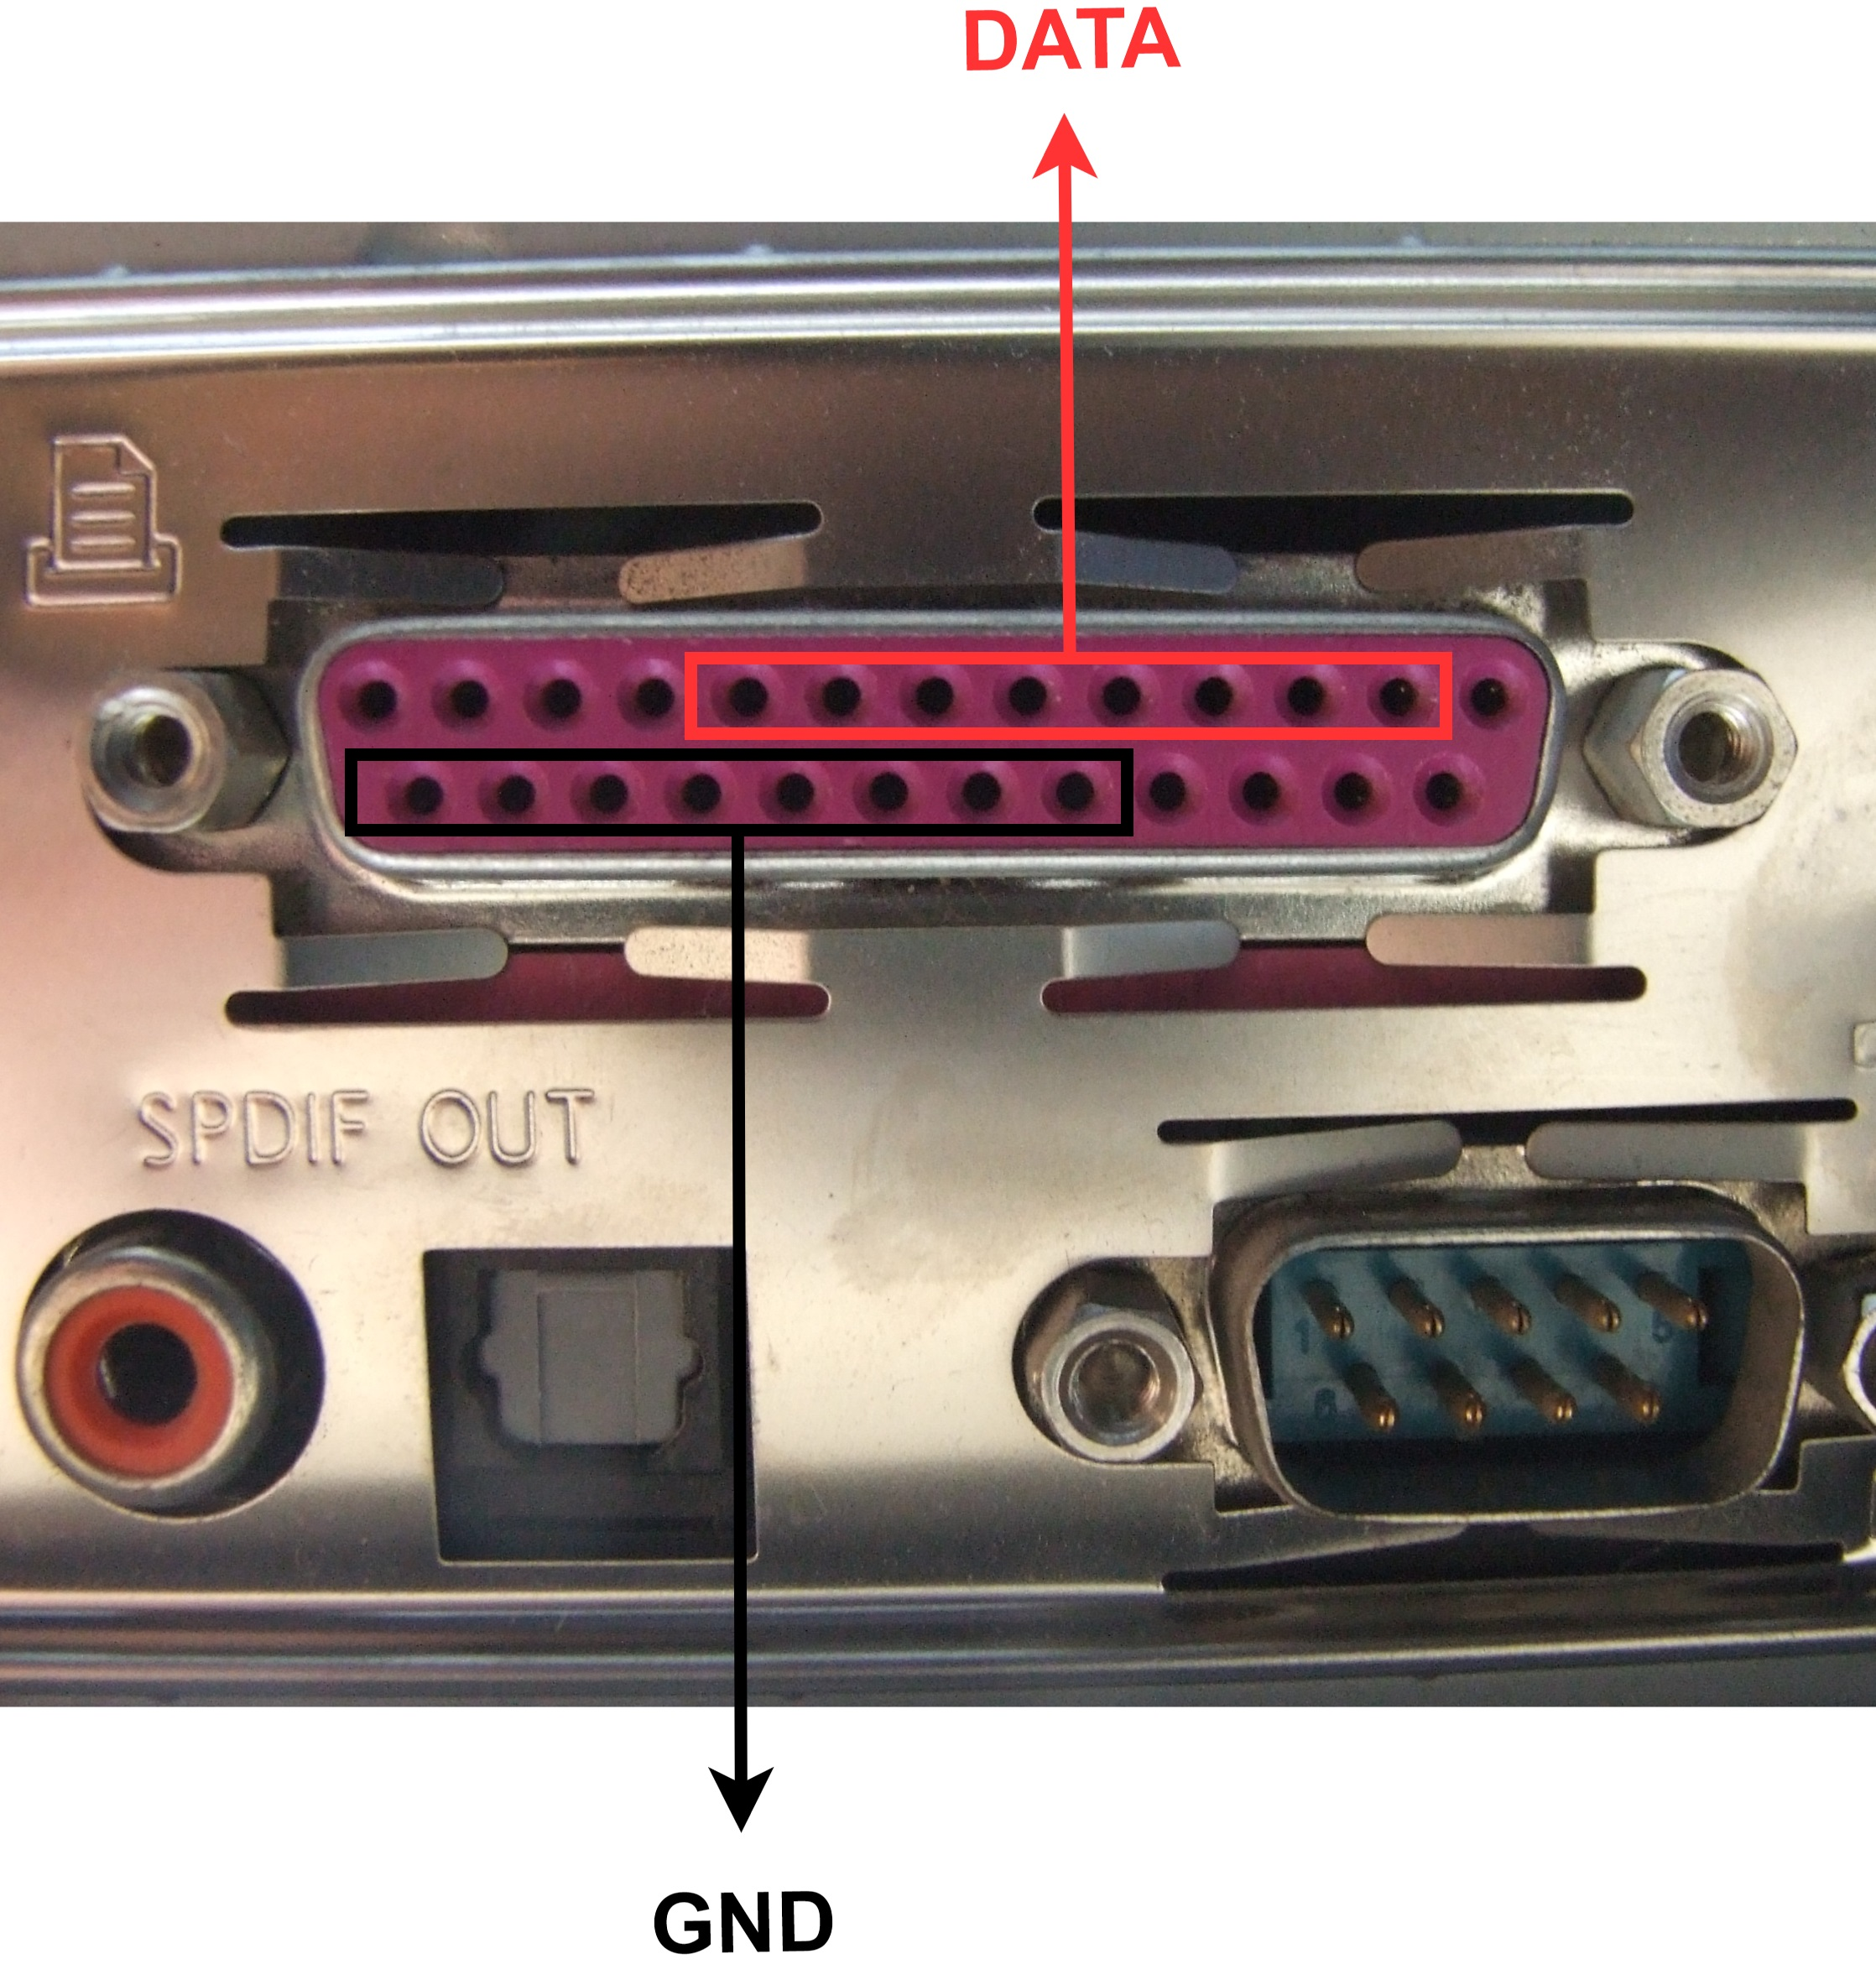
\includegraphics[width=8cm]{par_port}
\caption{Parallel port pins: DATA and GND.}				
\label{fig:par_port}
\end{figure}

You should be mostly interested in two sets of pins on the parport - data pins (DATA) and ground pins (GND). There's eight data pins, marked in red in the picture above. They will serve as our (+) and they are the ones, who's high and low states can be controlled from the program. There's also eight ground pins, marked in black in the picture and they serve as our (-).

It doesn't really matter which ground pin you connect to. It also doesn't matter which data pin you connect to but you should adjust the number of that pin, entering new value in the place of \verb|yourNewPinNumber| in the file \verb|sendToPort.cpp|:

\begin{snugshade}
\verb|ioperm(base, yourNewPinNumber, 1)|
\end{snugshade}


We have connected to the zero$^{th}$ data pin.

You should also be equiped with a parallel port plug. The best idea is to solder ground and data cables so that they stick firmly to the plug. Here's the picture of our plug, connected to the cables:

\begin{figure}[H]
\centering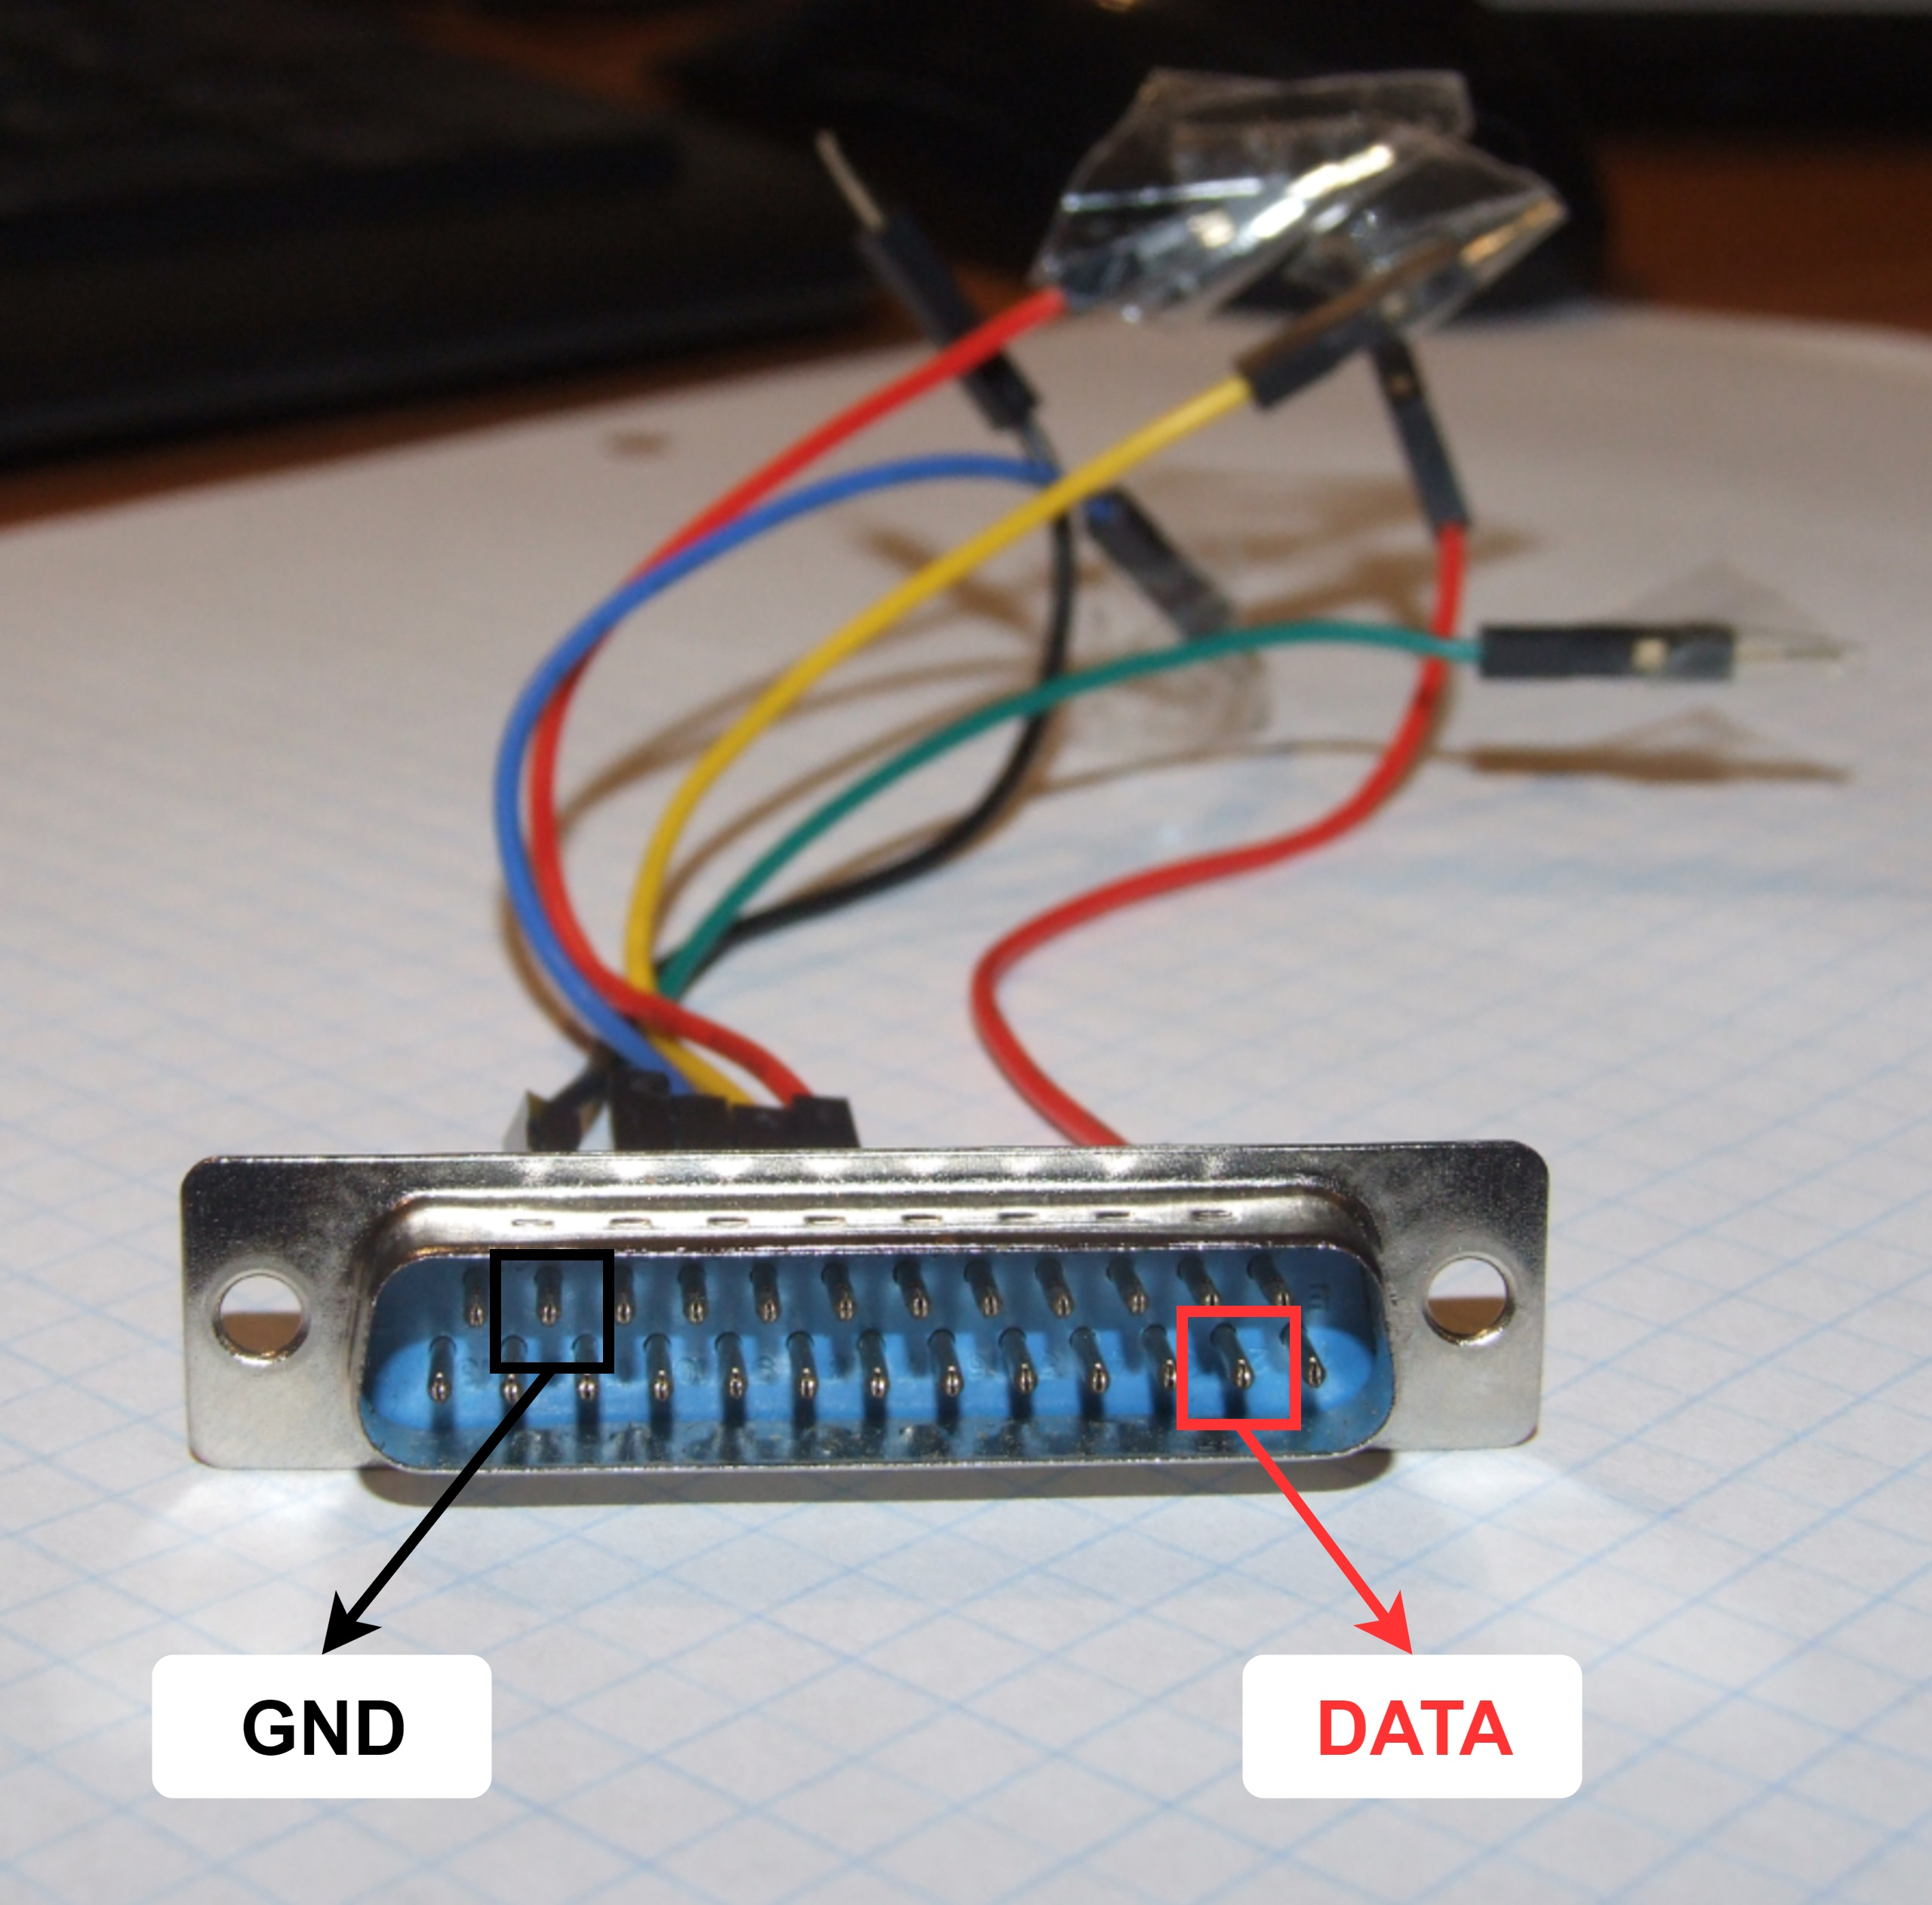
\includegraphics[width=8cm]{parport_plug}
\caption{Parallel port plug.}				
\label{fig:parport_plug}
\end{figure}

Remember that you only need two cables - one ground and one data. You don't have to worry about other cables present in the picture above.

The final thing to do is to build the rest of the circuit connected to the plug, which is very simple! It only consist of an LED diode and a 330$\Omega$ resistor.

\begin{figure}[H]
\centering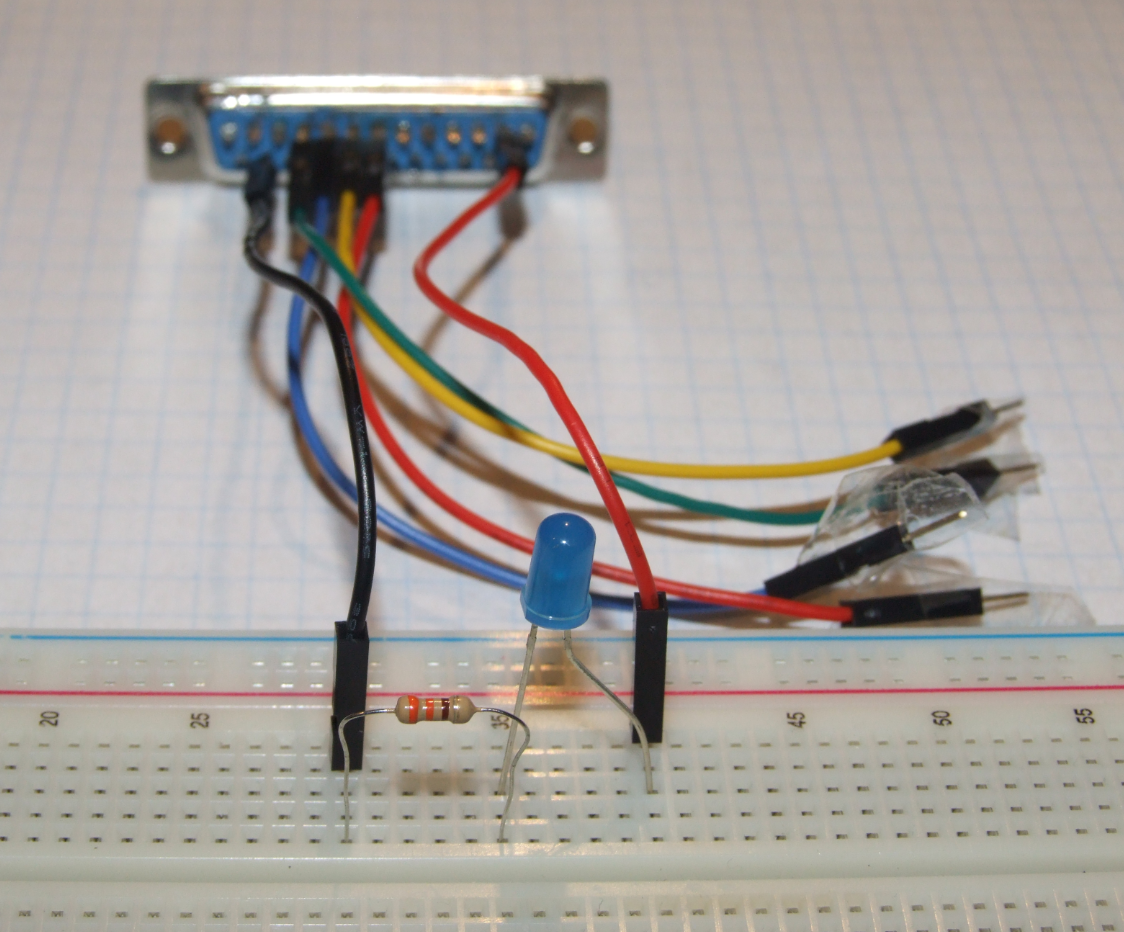
\includegraphics[width=8cm]{broadcast_circuit}
\caption{Electronic circuit for broadcasting.}				
\label{fig:broadcast_circuit}
\end{figure}




\subsection{Alphanumeric to Morse} \label{sec:asciitomorse}

Probably the most important part of the \textbf{broadcasting} phase is the introduction of the Morse alphabet in the code. Each letter \verb|A-Z| (\verb|a-z|) and each digit \verb|0-9| has got its representative in the Morse alphabet. Its definition is present in the file \verb|morse.cpp|. Notice that the Morse alphabet is not case sensitive and both lower-case and upper-case letters translate into the same Morse character.

We created an array of strings called \verb|morse::code| that contains the Morse alphabet. Its graphical representation is shown below:

\begin{figure}[H]
\centering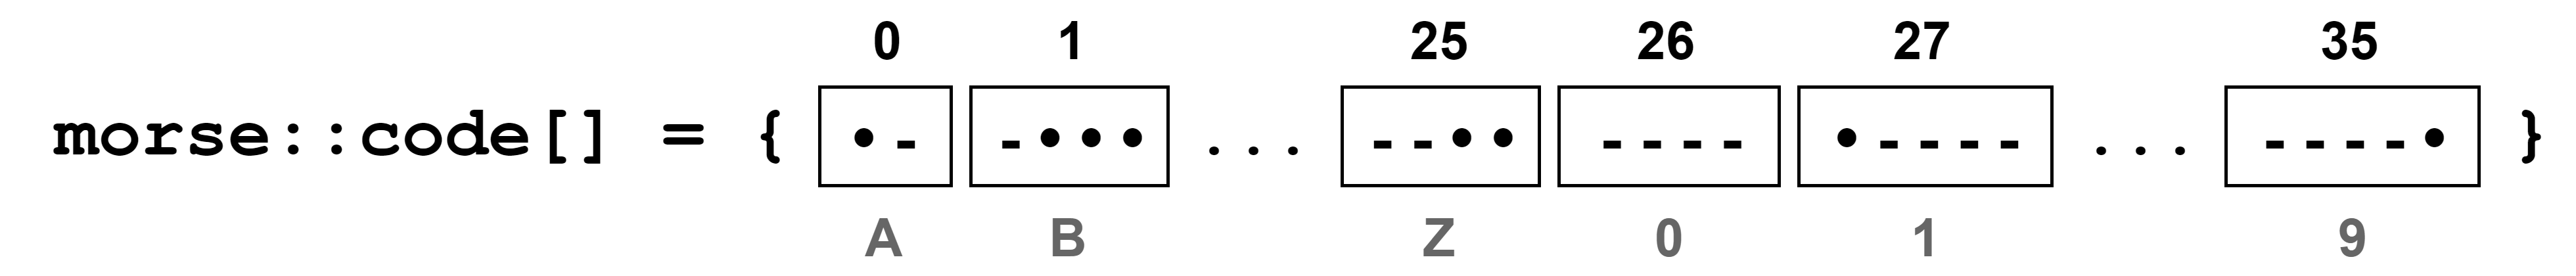
\includegraphics[scale=0.1]{morse--code}
\caption{Morse code array.}				
\label{fig:morse_code_array}
\end{figure}

Every ASCII character is assigned a number, which inside of a C++ code can be retrieved by casting the character into the integer. This is done by the following line: 

\begin{snugshade}
\verb|num = (int)textMessage[n];|
\end{snugshade}

For example, for a \verb|textMessage| character equal to "\verb|f|" the parameter \verb|num| will be equal to 102.

For the characters used in this project we have the following ASCII numerations:


\begin{enumerate}

\item upper-case letters \verb|A-Z| : 65 - 90

\item lower-case letters \verb|a-z| : 97 - 122

\item digits \verb|0-9| : 48 - 57

\item space \verb|" "| : 32

\item dot \verb|"."| : 46

\item comma \verb|","| : 44

\end{enumerate}


We have then decided to map every legal alphanumeric ASCII character into the created array. This means that each alphanumeric character number gets the number of its position inside the \verb|morse::code| array. This is achieved by subtracting certain number from the ASCII numeration. The graphical representation of this mapping is presented below:

\begin{figure}[H]
\centering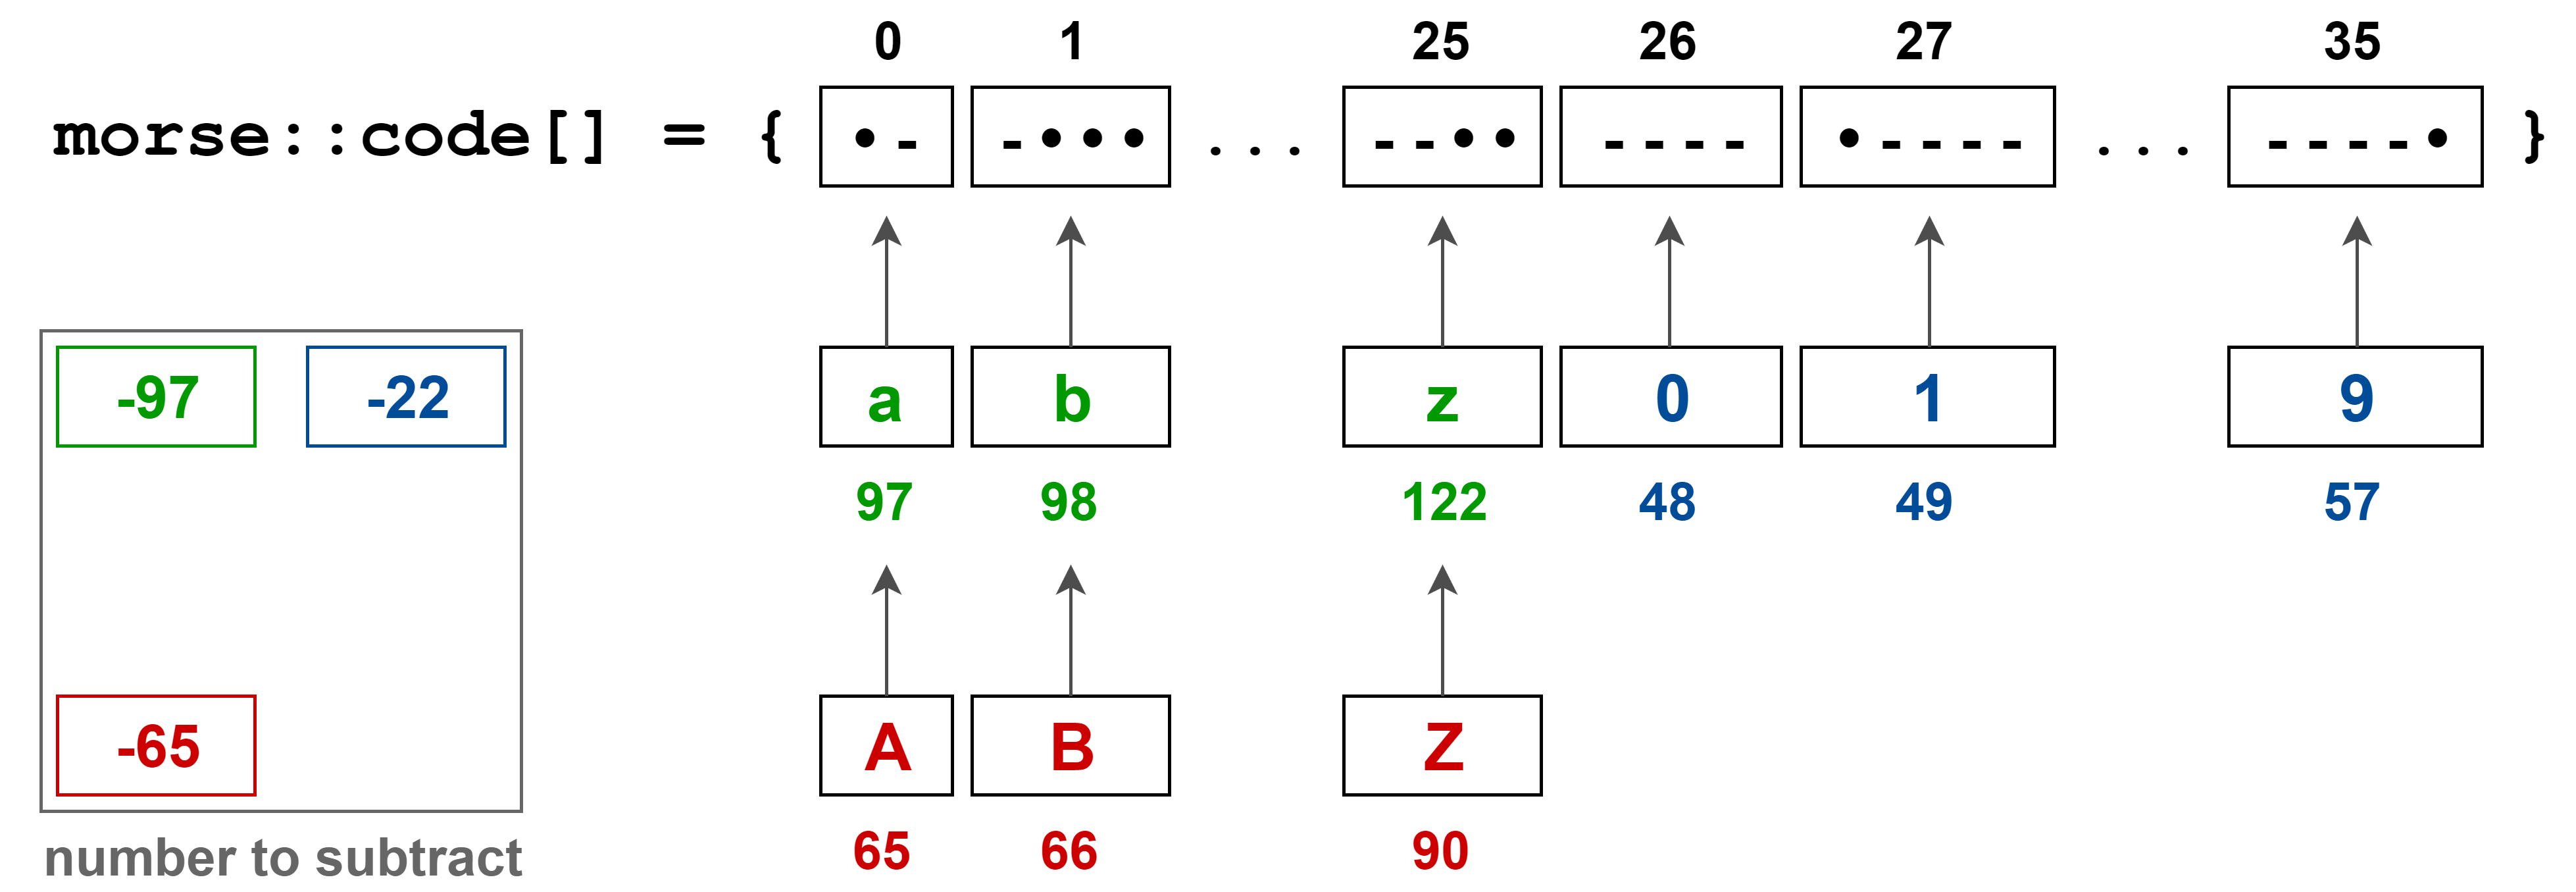
\includegraphics[scale=0.1]{morse_code_map}
\caption{Mapping alphanumeric characters to the morse code array.}				
\label{fig:morse_code_map}
\end{figure}

Inside of the code we have therefore:

\begin{snugshade}
\begin{verbatim}
if (num > 64 && num < 91) morseMessage += code[num - 65];
else if (num > 47 && num < 58) morseMessage += code[num - 22];
else if (num > 96 && num < 123) morseMessage += code[num - 97];
\end{verbatim}
\end{snugshade}

Using our previous example, the character "\verb|f|" will result in \verb|num| = 102, and since this number is between 96 and 123 (lower-case character), the number subtracted will be 97. This will altogether result in the position with index 5 in the \verb|morse::code| array, which corresponds to a string "$\cdot\cdot$\text{-}$\cdot$". 

This string will be added (\verb|+=|) to the message translation variable \verb|morseMessage|.

And so with each run of the \verb|for| loop, the coded message will be appended by the next corresponding Morse code character.

Notice that there is also an \verb|else| statement, which takes care of other non-alphanumeric characters which the user can type. The legal non-alphanumeric characters includes a dot, a space and a comma. Every other character is by default replaced with a space in the translation.


\begin{snugshade}
\begin{verbatim}
else
{
	switch (num)
	{
		case 46:
		{
		morseMessage+="/";
		break;
		}
		case 32:
		{
		morseMessage+=" ";
		break;
		}
		case 44:
		{
		morseMessage+="/";
		break;
		}
		default:
		{
		morseMessage+=" ";
		break;
		}
	}
}
\end{verbatim}
\end{snugshade}


\newpage

\chapter{Receiving}

\verb|OBJECTIF_MORSE, PHASE: RECEIVING -|


\section{Code description}


\section{How does it work}





\subsection{Arduino part}



\subsubsection{Initials}

The aim of the Arduino code is to identify the signal as Low or High and to measure the time duration of that state. One of the sample Arduino outputs is therefore:

\begin{snugshade}
\begin{verbatim}
L 200
H 200
L 400
H 200
L 200
H 400
\end{verbatim}
\end{snugshade}

Which has the interpretation as follows: Low state lasted 200ms, High state lasted 200ms, Low state lasted 400ms, and so on...




\subsubsection{Variables}

Variables used in the code:

\verb|analogInPin| - specifies the analog pin that we connect to, in our case it's A0.

\verb|sensorValue| - the value of voltage read using \verb|analogRead()| function. This value describes the luminosity change and comes directly from the phototransistor circuit. It's a number between 0 and 1023.

\verb|sensorMean| - the mean luminosity, assuming that the LED diode is not lit up. It is calculated in the calibration part of the code.

\verb|sensorThres| - the upper threshold of the Low state. Any value higher then this will be considered a High state. It is calculated in the calibration part of the code.

\verb|prevSignal| - a boolean describing the state from which the switch has just occured. It is \verb|true| when the previous state was High and \verb|false| when the previous state was Low.

\verb|timeDuration| - 

\verb|timePrev| - 










\subsubsection{Calibration}

The aim of the calibration is to measure the mean luminosity around the phototransistor and to use this information for further processing of the luminosity that comes from the LED diode itself. 

The need to do this comes from the fact that we can send our coded messages during sunny or gloomy day or during the night, and we want Arduino to correctly interpret what part of the luminosity comes from the general brightness of the day (or night) and what part will be changes due to the LED diode broadcasting the message.

\subsubsection{Identifying the voltage changes}







\chapter{Remarks}

- reading secret alien messages

- laser beam




\newpage


\begin{thebibliography}{50}

\end{thebibliography}

\end{document}
